\chapter{System Characterization}
\label{ch:sys-char}

\section{System Model}
\label{sec:system-model}

The hardware system is represented by a graph $G_s = \{E,V\}$ where $E$ is a set of edges representing communication links, and $V$ is a set of vertices representing communication endpoints, or data routing elements.
Sections~\ref{sec:system-vertices} and \ref{sec:system-edges} describe the specific system components explored.
Associated with each edge is a performance model function $M: C \rightarrow P$ that maps communication $C$ to an achievable performance $P$.

The communication $C$ has the following parameters:
\begin{itemize}
    \item The communication API or method used (e.g., \texttt{fread()}, CUDA unified memory page transfer).
    \item The size of the communication.
\end{itemize}

% The link utilization $U$ a set of extant communication patterns already sharing the link, separate from the communication of interest $C$.

Each vertex in $V$ is a data routing element.
These vertices are able to receive and re-transmit data on any of their links.
A PCIe hub \todo{cite PCIe discussion} is an example of a pure data-routing vertex.
Optionally, the vertex may serve as a communication endpoint; a source or a sink for data.
Processing elements and data storage elements serve as communication endpoints.


\texttt{hwcomm}~\cite{pearson2018hwcomm} is an open-source tool developed for automated hardware topology enumeration and characterization.
This tool can be executed on a target system to generate $G_s$ for that system.
Presently, the tool has only been tested on Linux operating systems.



%
% SECTION
%
\section{\texttt{hwcomm} Topology Enumeration}
\label{sec:topology-exploration}

The first step in generating $G_s$ is to discovere the topology.
hwcomm builds an in-memory representation of $G_s$, with sufficient information to later access the device during characterization.
Enumeration is done in several phases.

\textbf{Enumerate and Link CPU Sockets:}

First, the Portable Hardware Locality~\cite{broquedis2010hwloc} (hwloc) library is used to enumerate the present CPU sockets.
As the test systems only have two sockets, all discovered sockets are considered to be directly connected by an SMP bus for the appropriate system type.
The sockets and SMP busses are added to $G_s$.
\todo{more detail? list all information recorded?}

\textbf{Enumerate PCI devices:}

Next, hwloc is used to traverse the PCI device tree.
All PCI devices are added to $G_s$ and connected with PCI links of the appropriate type.
Most attached storage, networking, and computing components are assigned an address in the PCI system and are discoverable in this step.

\todo{more detail? list all information recorded?}

\textbf{Update GPUs to NVIDIA GPUs as appropriate:}

Next, the NVIDIA Management Library~\cite{nvidia2017nvml} (NVML) is used to enumerate all NVIDIA GPUs.
Those GPUs are matched by PCI address with existing PCI devices previously added to $G_s$, and NVML is used to discover whether NVLink is supported on each GPU and which other device that NVLink terminates at.
THis information is not provided by hwloc.
The edges associated with those NVLinks are added to $G_s$.
\todo{more detail? list all information recorded?}


\textbf{Enumerate Linux block devices:}

Linux block devices are enumerated through \todo{more detail} and added to $G_s$.
Where applicable, enough information about the device is stored within the vertex to be able to access the device later for characterization.
\todo{more detail? list all information recorded?}

\textbf{Enumerate Linux network devices:}

Finally, network devices are enumerated through \todo{more detail} and added to $G_s$.
Where applicable, enough information about the device is stored within the vertex to be able to access the device later for characterization.
\todo{more detail? list all information recorded?}

\subsection{Vertex Types}
\label{sec:system-vertices}

Table~\ref{tab:topology-vertices} summarizes the types of data routers discovered by hwcomm.
These make up the vertices of $G_s$.

\begin{table}[]
    \centering
    \caption[Discoverable vertex types]{
        A summary of the types of data routers that can be discovered by \texttt{hwcomm}.
        Some components may also serve as data endpoints.
        }
    \label{tab:topology-vertices}
    \begin{tabular}{|c|c|c|}
    \hline
    \textbf{Hardware}       & \textbf{Data Endpoint} & \textbf{Description} \\ \hline
    CPU Socket              &  \checkmark            &                \\ \hline
    PCI Device              &  \checkmark            &                \\ \hline
    PCIe Hostbridge         &                        &                \\ \hline
    PCIe Bridge             &                        &                \\ \hline
    CUDA GPU                & \checkmark             &                \\ \hline
    Linux Block Device      & \checkmark             &                \\ \hline
    Linux Network Interface & \checkmark             &                \\ \hline
    \end{tabular}
\end{table}

\subsection{Edge Types}
\label{sec:system-edges}

In $G_s$, the vertices are connected by the discoverable edge types shown in Table~\ref{tab:topology-edges}.

\begin{table}[]
    \centering
    \caption[Discoverable edge types]{
        A summary of the types of communication links that can be discovered by \texttt{hwcomm}.
        Some components may also serve as data endpoints.
    }
    \label{tab:topology-edges}
    \begin{tabularx}{\linewidth}{ |c | >{\centering\arraybackslash}X |}
    \hline
    \textbf{Edge Type} & \textbf{Description} \\ \hline
    SMP Bus            & A symmetric multiprocessing bus connecting two CPU sockets. \\ \hline
    PCIe Bus           & A PCIe link connecting a PCIe Bidge and PCIe device or PCIe Hostbridge and PCIe bridge. \\ \hline
    NVLink1            & A first-generation NVLink connecting two NVIDIA GPUs or an NVIDIA GPU and CPU \\ \hline
    NVLink2            & A second-generation NVLink connecting two NVIDIA GPUs or an NVIDIA GPU and CPU \\ \hline
    SATA bus           & A Serial AT Attachment link conneting a host bus to a mass storage device. \\ \hline
    \end{tabularx}
\end{table}



%
% SECTION
%
\section{Link Characterization}
\label{sec:link-char}

After the system graph $G_s$ has been generated, the next task is to characterize the communication capabilities of the system.
The goal of this characterization is to determine the rate at which data of a particular size can be moved between devices.
Ideally, this characterization would occur on a per-link basis along each available path between two communicating devices.
In practice, the communication between many devices is mediated by APIs exposed by the operating system or vendor library.
These APIs abstract away some complexity from the data movement.

\begin{figure}
    \centering
    \begin{tikzpicture}[
        cpunode/.style={circle, draw=green!60, fill=green!5, very thick, minimum size=7mm},
        gpunode/.style={rectangle, draw=red!60, fill=red!5, very thick, minimum size=5mm},
        blocknode/.style={rectangle, draw=red!60, fill=red!5, very thick, minimum size=5mm},
        ]
        %Nodes
        \node[cpunode]   (s0)                  {Socket0};
        \node[blocknode] (b0)    [below=of s0] {Disk0};
        \node[cpunode]   (s1)    [right=of s0] {Socket1};
        \node[gpunode]   (g0)    [below=of s1] {GPU0};

        %Lines
        \path[-] (s0.east)  edge node [above] {SMP}    (s1.west);
        \path[-] (s0.south) edge node [left]  {PCIe0}  (b0.north);
        \path[-] (s1.south) edge node [right] {PCIe1}  (g0.north);
    \end{tikzpicture}
    \caption[A simple example topology]{\todo{clean this up}\todo{long caption}}
    \label{fig:simple-topology}
\end{figure}

For example, consider the simple example system topology in Figure~\ref{fig:simple-topology}.
If a CPU thread running on CPU1 calls \texttt{fread()} to move a block of data from Disk0 to the memory associated with CPU1, the OS will transparently move that data along the PCIe0 and SMP0 links.
Since this is the capability is exposed to applications, it is useful to characterize it as well, not just the intermediate PCIe0 and SMP links.

An overview of the characterization algorithm is shown in Algorithm~\ref{alg:link-char}.

\begin{algorithm}[ht]
    \SetAlgoLined
    \KwResult{Characterization of all links between all vertices in $G_s$ }
     Build $G_s$ as described in Section~\ref{sec:topology-exploration}\;
     \For{$v_1$ in $V$}{
         \For{$v_2$ in $V$}{
             \If{$v_1 \ne v_2$}{
                Chars $\gets$ SupportedCharacterizers($v_1$,$v_2$)\;
                \For{c in Chars} {
                    c($v_1$, $v_2$)\;
                }
             }
         }
     }
     \caption{Link characterization.}
     \label{alg:link-char}
\end{algorithm}

For each pair of vertices, \todo{hwcomm} determines whether direct communication between those vertices is supported by the operating system or vendor libraries.
For vertices with a path of more than one link between them (e.g. Disk0 to Socket1 in Figure~\ref{fig:simple-topology}) those individual links will be characterized separately.
For vertices with multiple paths between them, the characterized path will be implicitly chosen by the applied characterization method.
There may be multiple different communication modes between two verticies.
hwcomm implements multiple workloads to characterize those modes.

\begin{table}[]
    \centering
    \caption[\texttt{hwcomm CUDA} characterization workloads]{
        \texttt{hwcomm CUDA} characterization workloads.
        These workloads all move a fixed amount of data from the source device to the destination device.
        Depending on the source and destination device, different methods of moving data are available through CUDA.
    }
    \label{tab:cuda workloads}
    \begin{tabular}{|c|c|c|c|}
    \hline
    \textbf{Source Allocation} & \textbf{Destination Allocation} & \textbf{Transfer Method} & \textbf{Further Reading} \\ \hline 
    GPU                 & GPU          & cudaMemcpy, peer-enabled  & \ref{sec:gpu-gpu-peer} \\ \hline
    GPU                 & GPU          & cudaMemcpy, peer-disabled & \ref{sec:gpu-gpu-peer} \\ \hline
    GPU                 & GPU          & direct, from dst          & \ref{sec:gpu-gpu-direct} \\ \hline
    GPU                 & CPU Pageable & cudaMemcpy                & \ref{sec:gpu-cpu} \\ \hline
    GPU                 & CPU Pinned   & cudaMemcpy                & \ref{sec:gpu-cpu} \\ \hline
    CPU Pageable        & GPU          & cudaMemcpy                & \ref{sec:gpu-cpu} \\ \hline
    CPU Pinned          & GPU          & cudaMemcpy                & \ref{sec:gpu-cpu} \\ \hline
    CPU Write Combining & GPU          & cudaMemcpy                & \ref{sec:wc-gpu} \\ \hline
    CPU Mapped          & GPU          & direct                    & \ref{sec:cpu-gpu-direct} \\ \hline
    \end{tabular}
\end{table}

\subsection{GPU to GPU with cudaMemcpyPeer}
\label{sec:gpu-gpu-peer}

Both peer enabled and disabled.

\outline{ \\
    description \\
    required cuda / system support \\
    when is preferable \\
}





\subsubsection{OpenMP Socket to Socket Bandwidth}

The symmetric multi-processing links between CPU sockets are characterized by a synthetic workload generated using OpenMP~\cite{openmp2013}.
This workload creates multiple threads reading remote data in an attempt to saturate the socket memory controllers and SMP bus.
Algorithm~\ref{alg:h2h} describes the approach.

\begin{algorithm}[ht]
    \SetAlgoLined
    \KwResult{bandwidth vs. transfer size between CPU sockets $src$ and $dst$}
    numThreads $\gets$ 10\;
    \todo{Choice of elemSize}\;
    \For{poolSize $\gets$ 128 to sweepFinish} {
        bind process to $src$\;
        bind memory allocation to $src$\;
        \For{tid $\gets$ 0 := numThreads}{
            regions[tid] $\gets$ alloc(poolSize)\;
        }
        bind process to $dst$\;
        start OpenMP parallel region\;
        start $\gets$ wall\_time()\;
        \texttt{sum\_array(region[omp\_get\_thread\_num(), elemSize])}\;
        stop $\gets$ wall\_time()\;
        bandwidth $\gets$ $\frac{copySize}{stop - start}$\;
    }
    \caption{Synthetic workload for testing SMP bus.}
    \label{alg:h2h}
\end{algorithm}

\texttt{sum\_array()} is a function used to ensure that every data element is accessed, and the compiler does not optimize out the otherwise unused remote data read.
\texttt{sum\_array()} adds the elements in the region using loads and accumulates of a desired size.

%
% SECTION
%
\section{System Characterization Case Studies}

The system characterization was executed on two high-performance heterogeneous systems: an IBM S822LC ``Minsky''~\cite{ibm2015minsky}, and an NVIDIA DGX-1~\cite{nvidia2016dgx1}.
The two systems both feature 512 GB of system memory, two multi-core GPUs, and multiple NVIDIA Tesla P100 GPUs.
Their key differences are in CPU architecture (ppc64le for ``Minsky'', x86-64 for DGX-1), number of GPUs (4 vs 8), and GPU connection topology (bonded NVLink vs hybrid PCIe/NVLink).

\subsection{IBM S822LC ``Minsky''}
\label{sec:topology-minsky}

\begin{table}[]
    \centering
    \caption[Minsky hardware summary.]{
        Brief summary of Minsky hardware.
        }
    \label{tab:minsky}
    \begin{tabular}{|c|c|}
    \hline
    \textbf{} & \textbf{Specification}                  \\ \hline
    CPU               &  \makecell{2x IBM Power8 \\ 20C / 80T \\ 4 GHz}  \\ \hline
    System Memory     &  512 GB DDR4                          \\ \hline
    GPU               &  4 NVIDIA P100                        \\ \hline
    \end{tabular}
\end{table}

The IBM S822LC ``Minsky'' machine features two Power8 CPUs and four NVIDIA P100 GPUs.
Each Power8 CPU is part of a fully-connected triad of one Power8 CPU and two P100 GPUs.
Each device in the triad is connected by two NVLinks.
The two triads are connected at the Power8 CPUs by an IBM SMP bus\todo{cite}.
Table~\ref{tab:minsky} summarizes the hardware configuration.

The IMB ``Minsky'' machine consists of two symmetric sections, connected by an IBM X bus between two 10-core Power8+ CPUs with 8-way simultaneous multithreading (SMT).
Each CPU is connected to 256GB of DDR3 RAM.
Each CPU is also connected to two NVIDIA Tesla P100 GPUs by two bonded NVLink blocks.
Those P100s within the symmetric section are also connected to each other by two bonded NVLinks.
The second CPU socket hosts the majority of the PCI devices on the system, including the network interfaces and the disks.
Figure \ref{fig:topo-minsky-simple} shows a simplified view\footnote{Figure \ref{fig:topo-minsky-actual} shows a detailed view.} of the topology discovered by \todo{hwcomm}.


\begin{figure}
    \centering
    \begin{tikzpicture}[
        cpunode/.style={circle, draw=green!60, fill=green!5, very thick, minimum size=7mm},
        gpunode/.style={rectangle, draw=red!60, fill=red!5, very thick, minimum size=5mm},
        blocknode/.style={rectangle, draw=red!60, fill=red!5, very thick, minimum size=5mm},
        nvlink/.style={>={latex[length=10pt]}, <->, very thick, double distance=2pt, shorten <=2pt, shorten >=2pt},
        smp/.style={>={latex[length=10pt]}, <->, very thick, double distance=2pt, shorten <=2pt, shorten >=2pt},
        ]
        %Nodes
        \node[cpunode]   (s0)                  {Socket0};
        \node[cpunode]   (s1)    [right=4cm of s0] {Socket1};
        \node[gpunode]   (g0)    [below=2cm of s0] {GPU0};
        \node[gpunode]   (g1)    [left=2cm of g0]  {GPU1};
        \node[gpunode]   (g2)    [below=2cm of s1] {GPU2};
        \node[gpunode]   (g3)    [right=2cm of g2] {GPU3};

        %Lines
        \path[] (s0.east)  edge [smp] node [above] {SMP}    (s1.west);

        \path[] (s0.south) edge [nvlink] node [left]  {NVLink}  (g0.north);
        \path[] (s0.west)  edge [nvlink] node [left]  {NVLink}  (g1.north);
        \path[] (g0.west)  edge [nvlink] node [below] {NVLink}  (g1.east);

        \path[] (s1.south) edge [nvlink] node [left]  {NVLink}  (g2.north);
        \path[] (s1.east)  edge [nvlink] node [right] {NVLink}  (g3.north);
        \path[] (g2.east)  edge [nvlink] node [below] {NVLink}  (g3.west);
    \end{tikzpicture}
    \caption{IBM ``Minsky'' simplified topology.}
    \label{fig:topo-minsky-simple}
\end{figure}

\begin{figure}[ht]
    \centering
    \begin{subfigure}[b]{0.3\textwidth}
        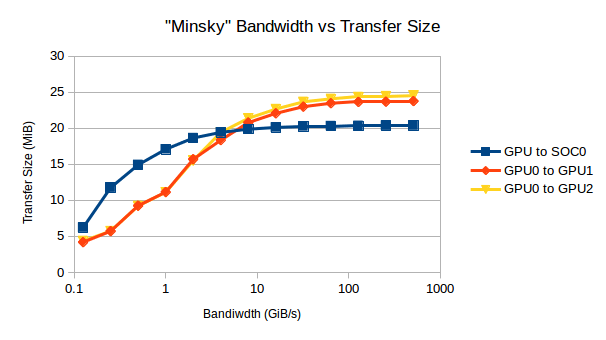
\includegraphics[width=\textwidth]{figures/minsky-soc0-gpu0.png}
        \caption{A gull}
        \label{fig:gull}
    \end{subfigure}
    ~
    \begin{subfigure}[b]{0.3\textwidth}
        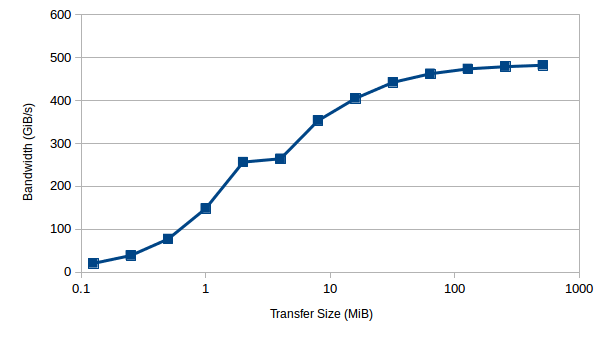
\includegraphics[width=\textwidth]{figures/minsky-gpu0-gpu0.png}
        \caption{A gull}
        \label{fig:gull}
    \end{subfigure}

    \caption[\todo{short}]{\todo{long}}
    \label{fig:minksy}
\end{figure}

\subsection{NVIDIA DGX-1}
\label{sec:topology-dgx1}

The NVIDIA DGX-1 machine consists of two symmetric sections.
Each section consists of one 20-core Intel Xeon E5-2698v4 CPUs with 2-way SMT.
Each CPU is connected to 256GB of DDR4 RAM.
Each section has 4 NVIDIA Tesla P100 GPUs coupled by single NVLinks.
The sections are connected by an Intel QPI bus between the CPUs, as well as NVLinks between corresponding GPUs.
The first CPU socket hosts the majority of the PCI devices on the system, including the network interfaces and the disks.
Figure \ref{fig:topo-dgx-simple} shows a simplified view\footnote{Figure ~\ref{fig:topo-dgx-actual} shows a detailed view.} of the topology discovered by \todo{hwcomm}.


\begin{figure}
    \centering
    \begin{tikzpicture}[
        cpunode/.style={circle, draw=green!60, fill=green!5, very thick, minimum size=7mm},
        gpunode/.style={rectangle, draw=red!60, fill=red!5, very thick, minimum size=5mm},
        blocknode/.style={rectangle, draw=red!60, fill=red!5, very thick, minimum size=5mm},
        ]
        %Nodes
        \node[cpunode]   (s0)                  {Socket0};
        \node[blocknode] (b0)    [below=of s0] {Disk0};
        \node[cpunode]   (s1)    [right=of s0] {Socket1};
        \node[gpunode]   (g0)    [below=of s1] {GPU0};

        %Lines
        \path[-] (s0.east)  edge node [above] {SMP}    (s1.west);
        \path[-] (s0.south) edge node [left]  {PCIe0}  (b0.north);
        \path[-] (s1.south) edge node [right] {PCIe1}  (g0.north);
    \end{tikzpicture}
    \caption{NVIDIA DGX-1 simple topology.}
    \label{fig:topo-dgx-simple}
\end{figure}

\subsection{Single-Socket x86 with NVIDIA P100 ``Blaise''}

\subsection{Dual-Socket Power9 and NVIDIA Volta V100 ``hal000''}

\section{Write-Combined Memory}

CPU bandwidth writing to wc memory

GPU bandwidth copying back to wc memory


\section{Observations}

Misnky2
\begin{itemize}
\item GPU-GPU coherence bandwidth depends on local/remote
\item GPU-GPU prefetch bandwidth depends on local/remote
\item CPU-GPU um bandwidth has crossover
\item GPU-CPU um bandwidth has crossover
\end{itemize}

Impact1
\begin{itemize}
    \item Pageable copy bandwidth faster than pinned
    \item WC bandwidth small for small transfers
\end{itemize}


\section{Extensions}
\subsection{cudaMemAdviseSetReadMostly}
\begin{itemize}
    \item CPU-GPU coherence bandwidth (r/w, x access patterns)
    \item GPU-GPU coherence bandwidth (r/w, x access patterns)
    \item estimate invalidation cost (CPU-GPU, GPU->GPU)
\end{itemize}

\subsection{System Atomics}
\begin{itemize}
    \item Latency and throughput for PCIe PASCAL / NVLink1 Pascal 
    \item Latency and throughput for PCIe Volta / NVLink2 Volta
\end{itemize}

\subsection{Multi-GPU Sync}
\begin{itemize}
    \item CUDA 9.1 / Power9 / NVLink2 / Volta
\end{itemize}


\section{Parking Lot}
\subsection{Volta access counters for triggering migration}
\begin{itemize}
    \item local CPU->GPU
    \item remote CPU->GPU
    \item local GPU->GPU
    \item remote GPU->GPU
\end{itemize}


\section{Atomics and Unified Memory}
\begin{itemize}
    \item effect oof cudaMemAdviseSetAccessedBy on imbalanced GPU/GPU atomics contention
\end{itemize}